\section{クラスタリング実験}

\subsection{実験環境}
実験にはPython3.5を用い,
機械学習のライブラリとしてTensorFlowを用いてアルゴリズムを実装した.

\subsection{K-meansによるクラスタリング}
\figref{img:kmeans-before}のデータをクラスタ数5としてクラスタリングした結果,
\figref{img:kmeans-after}のような結果になった.

% なお,クラスタリングの打ち切り条件は,セントロイドの差が$1.0\times10^{-10}$以下のときとした.
\begin{figure}[htbp]
  \begin{center}
    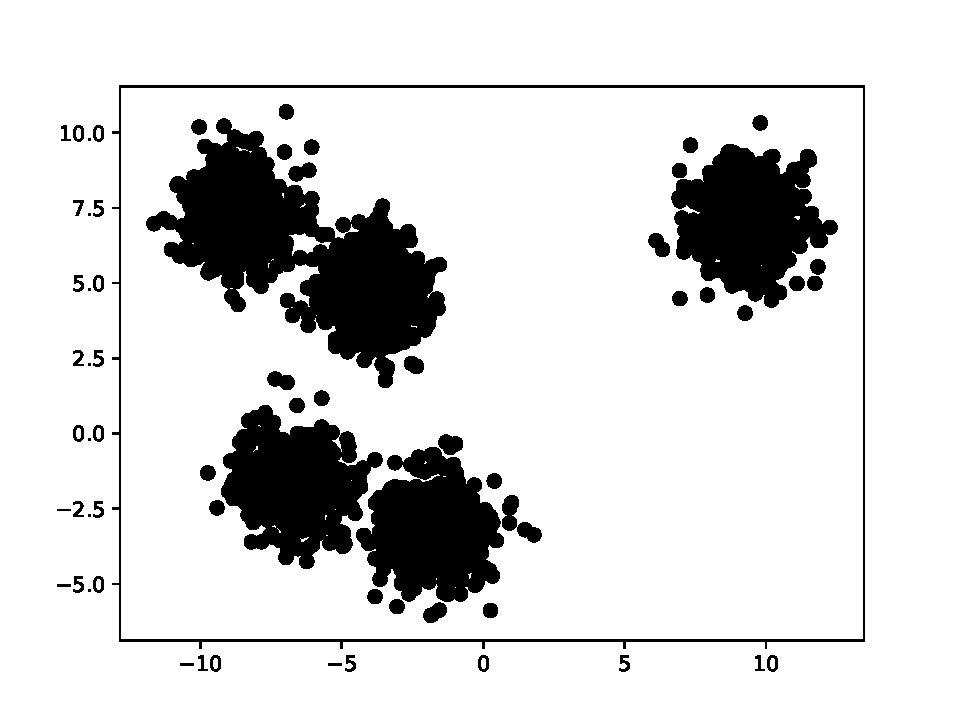
\includegraphics[width=0.8\linewidth]{img/k-means/before.pdf}
    \caption{クラスタリング前のデータ}
    \label{img:kmeans-before}
  \end{center}
\end{figure}
\begin{figure}[htbp]
  \begin{center}
    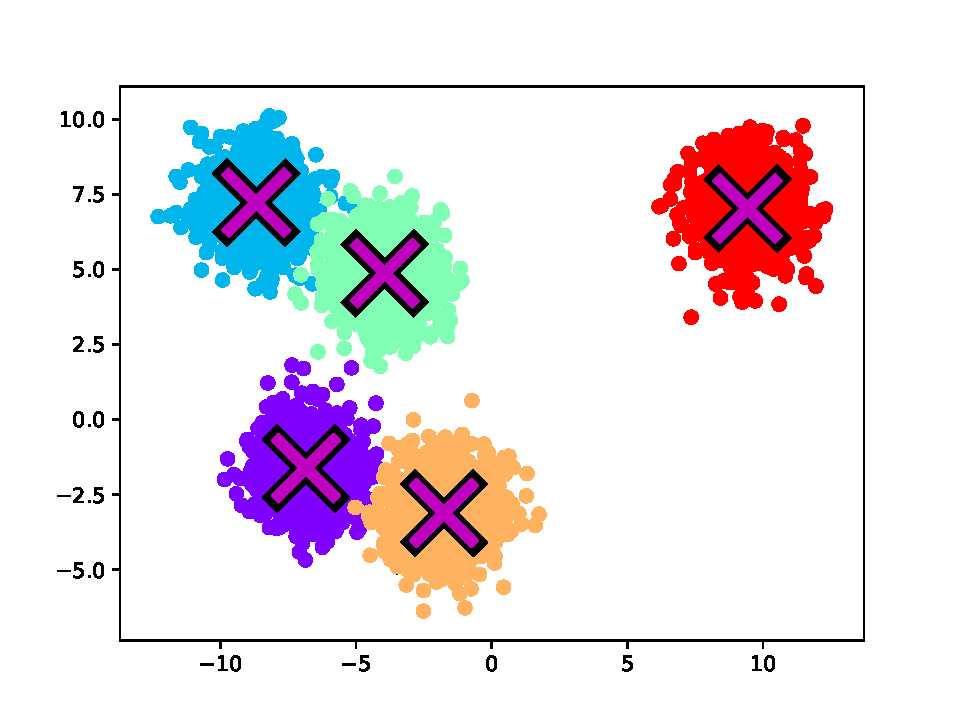
\includegraphics[width=0.8\linewidth]{img/k-means/after.pdf}
    \caption{K-meansによるクラスタリング結果}
    \label{img:kmeans-after}
  \end{center}
\end{figure}

\subsection{X-meansによるクラスタリング}
K-meansと同様に,クラスタ数が5つのデータを生成し,X-meansにより分割した結果,
\figref{img:xmeans-after}のようになった.
図より,クラスタ数を5つとして適切にクラスタリングを行っていることがわかる.

\begin{figure}[htbp]
  \begin{center}
    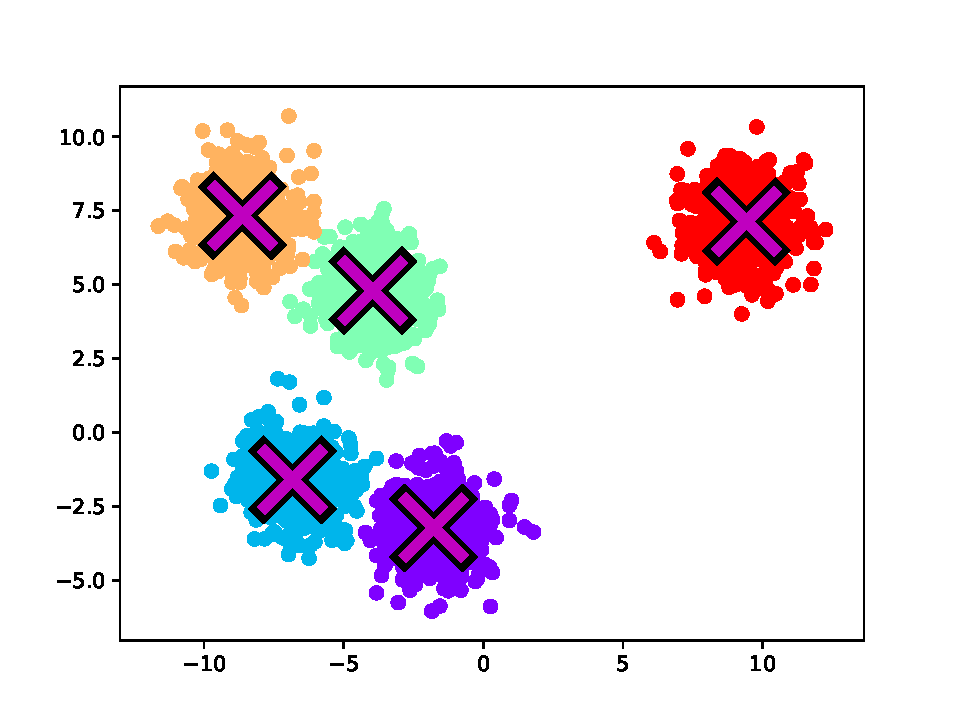
\includegraphics[width=0.8\linewidth]{img/x-means/after.pdf}
    \caption{X-meansによるクラスタリング結果}
    \label{img:xmeans-after}
  \end{center}
\end{figure}
